% 
% Annual Cognitive Science Conference
% Sample LaTeX Paper -- Proceedings Format
% 

% Original : Ashwin Ram (ashwin@cc.gatech.edu)       04/01/1994
% Modified : Johanna Moore (jmoore@cs.pitt.edu)      03/17/1995
% Modified : David Noelle (noelle@ucsd.edu)          03/15/1996
% Modified : Pat Langley (langley@cs.stanford.edu)   01/26/1997
% Latex2e corrections by Ramin Charles Nakisa        01/28/1997 
% Modified : Tina Eliassi-Rad (eliassi@cs.wisc.edu)  01/31/1998
% Modified : Trisha Yannuzzi (trisha@ircs.upenn.edu) 12/28/1999 (in process)
% Modified : Mary Ellen Foster (M.E.Foster@ed.ac.uk) 12/11/2000
% Modified : Ken Forbus                              01/23/2004
% Modified : Eli M. Silk (esilk@pitt.edu)            05/24/2005
% Modified : Niels Taatgen (taatgen@cmu.edu)         10/24/2006
% Modified : David Noelle (dnoelle@ucmerced.edu)     11/19/2014
% Modified : Roger Levy (rplevy@mit.edu)     12/31/2018



%% Change "letterpaper" in the following line to "a4paper" if you must.

\documentclass[10pt,letterpaper]{article}

\usepackage{cogsci}
\usepackage{color}
\usepackage{graphicx}
\graphicspath{{figs/}}
%\cogscifinalcopy % Uncomment this line for the final submission 

\usepackage{tikz}
\usepackage{tikz-qtree}
\usepackage{caption}
\usepackage{subcaption}
\usepackage{pslatex}
\usepackage{apacite}
\usepackage{amsmath}
\usepackage{float} % Roger Levy added this and changed figure/table
                   % placement to [H] for conformity to Word template,
                   % though floating tables and figures to top is
                   % still generally recommended!

%\usepackage[none]{hyphenat} % Sometimes it can be useful to turn off
%hyphenation for purposes such as spell checking of the resulting
%PDF.  Uncomment this block to turn off hyphenation.


%\setlength\titlebox{4.5cm}
% You can expand the titlebox if you need extra space
% to show all the authors. Please do not make the titlebox
% smaller than 4.5cm (the original size).
%%If you do, we reserve the right to require you to change it back in
%%the camera-ready version, which could interfere with the timely
%%appearance of your paper in the Proceedings.

\providecommand{\tightlist}{%
  \setlength{\itemsep}{0pt}\setlength{\parskip}{0pt}}
  
\definecolor{Red}{RGB}{255,0,0}
\definecolor{Green}{RGB}{10,200,100}
\definecolor{Blue}{RGB}{10,100,200}

\newcommand{\mh}[1]{{\textcolor{Blue}{[mh: #1]}}}
\newcommand{\rl}[1]{{\textcolor{Green}{[roger: #1]}}}

\newcommand{\denote}[1]{\mbox{ $[\![ #1 ]\!]$}}
\newcommand{\red}[1]{{\textcolor{Red}{#1}}}

\newcommand\Tstrut{\rule{0pt}{2.6ex}}       % "top" strut
\newcommand\Bstrut{\rule[-1ex]{0pt}{0pt}} % "bottom" strut
\newcommand{\TBstrut}{\Tstrut\Bstrut} % top&bottom struts

\newcommand{\key}[1]{\emph{#1}}

%\title{Syntactic expectations modulate pragmatic interpretations of generic sentences}
%\title{The structure of prior knowledge and syntax in generic language understanding}
\title{Incremental, non-monotonic understanding of conjunctive generic sentences}
 
\author{{\large \bf Michael Henry Tessler (tessler@mit.edu)} \\
  Department of Brain and Cognitive Sciences, MIT \\
  Cambridge, MA 02139 USA
  \AND {\large \bf Roger Levy (rplevy@mit.edu)} \\
  Department of Brain and Cognitive Sciences, MIT \\
  Cambridge, MA 02139 USA}


\begin{document}

\maketitle


\begin{abstract}

%A hallmark of human thinking is the ability to update our beliefs in the face of conflicting evidence. 
%Talk with the same person for long enough and you will be able to predict what they will say before they have said it.
%We investigate the interface between

Generic statements convey generalizations about categories, but how generic predications combine is unclear.
``Elephants live in Africa and Asia'' does not mean that individual elephants live on both continents.
Such conjunctive generics %about mutually exclusive properties (e.g., where each property applies to a distinct subset of the category) 
also pose interesting questions for theories of incremental processing because the meaning of the sentence can change part-way through: ``Elephants live in Africa'' would imply most or all do. 
%Such conjunctive generics about mutually exclusive properties (e.g., where each property applies to a distinct subset of the category) also pose interesting questions for theories of incremental processing because the meaning of the sentence can change part-way through. 
We extend a recently proposed computational model of generic language understanding with an incremental processing mechanism that makes novel predictions for partial interpretations of conjunctive generic sentences.
We test these predictions with two behavioral experiments. 
The results support a strong view of incrementality, wherein listeners  continuously use their expectations about where a speaker will go next with their utterance to update their beliefs.


%Generics permit exceptions (e.g., not all birds fly, and yet ``Birds fly'' is true) and adequately dealing with the exceptions is a problem for any model of generic language understanding. 
%Here, we examine an extreme case of exceptionality in generics: 
%We show how a recent model of generic language understanding that posits that the literal meaning of a generic is underspecified or uncertain can interpret conjunctive generics about mutually exclusive properties.  
%Furthermore, we extend this model to incorporate syntactic expectations about where a speaker will go next with her utterance.
%This joint syntactic--semantic/pragmatic model makes novel predictions for incremental interpretations of conjunctive generic sentences, which we test across three experiments.
%The success of this model highlights the deep connection between syntactic knowledge and pragmatic language understanding. 

\textbf{Keywords:} 
semantics; pragmatics; incremental processing; generics
\end{abstract}


% follow-up: paramteric manipulate the ME

%\section{Introduction}

%Penguins would be upset if we understood the statement ``Birds fly'' to apply to the entire category of birds. 


Much of what we come to learn about the world comes not from direct experience but from knowledge conveyed to us from others, often in the form of linguistic utterances. 
``Elephants eat 300 pounds of a food in a day'' succinctly conveys information extending beyond any particular moment in time or space (e.g., it could apply to any elephant, any day of the week). 
Utterances that communicate generalizations are called \emph{generic} utterances \cite{Carlson1977, genericBook}, and they are the foremost case study of rich, abstract knowledge conveyed in simple utterances \cite{Gelman2009}.

Generics are rife with philosophical puzzles that make it difficult to develop a unified, formal theory of their meaning \cite<for useful reviews:~>{genericBook, Nickel2016}.  One largely understudied puzzle concerns how generic predications combine.  To appreciate the complexity, consider the null hypothesis that generics convey a \key{prevalence} analogous to that conveyed by a majority quantifier like \emph{most} or \emph{all} (e.g., ``Most elephants eat 300 pounds of food in day'').  How can such an account treat a generic involving a conjunctive predication like ``Elephants live in Africa and Asia''?  No elephant actually lives on both continents; instead, the sentence should be understood as ``Elephants live in Africa, and elephants live in Asia'', but this is impossible if each individual generic sentence means that the majority hold the property \cite<i.e., it is impossible for more than half of elephants to live in Africa and more than half of elephants to live in Asia;>{Nickel2008}.  In this case, the prevalence required for endorsing a generic involving a conjunctive predication seems more lax than if only one of conjuncts were mentioned: ``Wugs live in Africa'' intuitively still conveys that most or all wugs live in Africa.
%\mh{Collective interpretation of ``all'', ``most'' doesn't run into the issues?}

The puzzle of understanding conjunctive generic sentences deepen when one considers that actual linguistic input is processed incrementally \cite<e.g.,>{Altmann1999}: listeners ubiquitously form expectations about the intended meaning before the speaker finishes their sentence \cite<e.g.,>{tanenhaus-etal:1995}.  For conjunctive generics about mutually exclusive properties, strongly incremental language understanding might produce non-monotonic interpretation updates: after the sentence prefix ``Elephants live in Africa\ldots'', a comprehender might infer a higher prevalence than after hearing the sentence completion ``\ldots and Asia''.  And if such non-monotonic updates occur, what types of linguistic input trigger them?  

In this paper we demonstrate and empirically test two predictions about generic interpretation that address these puzzles.  The first prediction derives from \citeA{Tessler2019:genLang}'s model of generics as involving probabilistic  vague language interpretation.  This model predicts that the interpretation of conjoined generic predications depends on prior beliefs about the relationship between the properties:  When comprehenders believe the properties are likely to be mutually incompatible (as in ``live in Africa and Asia''), they infer lower prevalence than when the properties are compatible.  Second, when this model is integrated with expectation-based probabilistic theories of syntactic processing \cite{hale:2001,Levy2008}, it predicts that comprehenders update their beliefs about property prevalence not just when encountering a second, conjoined property, but immediately upon encountering evidence that a second, conjoined property is likely to be forthcoming.  We test these predictions in two behavioral experiments that probe listeners' understanding of conjunctive generic sentences at different points mid-sentence, analogous to gating paradigms in psycholinguistics \cite{Grosjean1980}.  Our data confirm both predictions, suggesting that generic language interpretation interacts jointly with world knowledge and strongly incremental syntactic processing according to principles of probabilistic inference under uncertainty.
 
%Here, we combine a recent model of generic language understanding  \cite{Tessler2019:genLang} with an incremental parsing mechanism to begin to form beliefs about a speaker's intended meaning before the speaker has finished speaking.
%The basic, non-incremental model understands ``Elephants live in Africa and Asia” as meaning that some elephants live in Africa and that different ones live in Asia, in the case where listeners have prior knowledge suggesting against the existence of elephants that live on both continents (\emph{international elephants}).
%Furthermore, the enriched incremental model makes the prediction that part-way through generic sentences about conjunctive predicates (e.g., ``Elephants live in Africa''), a listener will form strong beliefs (i.e., \emph{all elephants live in Africa}) which later get non-monotonically updated once more information comes in (\emph{some live in Africa and some live in Asia}).
%A model that allows for full interactions between the levels of syntactic processing and pragmatic reasoning allows for even finer-grained interpretations. 
%We test such a model in a set of language understanding tasks where participants are asked to report their beliefs about the prevalence of a property in a category at different points in a sentence, analogous to gating paradigms in psycholinguistics \cite{Grosjean1980}.


%Recently, \cite{Tessler2019:genLang} proposed a theory of generic language wherein the meaning of a generic is \emph{underspecified} (or, vague) and Bayesian reasoning is used to resolve more precise meanings in context.


%Intriguingly, this model also predicts that (i.e., upon hearing only that ``Elephants live in Africa'') leads our model to believe that most, possibly all, elephants live in Africa, but when the sentence is completed (``. . . and Asia''), the model nonmonotonically updates its beliefs to the weaker \emph{some elephants live in Africa and others in Asia}. 


%Interpreting generics in a consistent way is a non-starter. 


%Theories that appeal to standard, formal semantic, quantificational truth conditions (e.g., generic means \emph{most} or \emph{all} relevant or normal members of the category have the property) employ mechanisms to implicitly restrict the \emph{relevant} set of robins to be females in the case of a property concerning reproduction such as \emph{laying eggs}\cite<e.g.,>{Cohen1999}. 
%(such as that of  where a generic ``Ks F'' means roughly that \emph{most of the relevant Ks F})

%Interpreting generics in a 
%Such restrictions, however, are too limiting when interpreting conjunctive predicates as in ``Elephants live in Africa and Asia''. 
% from knowledge about the kind of property under consideration (i.e., \emph{laying eggs} has to do with reproduction, so we are only talking about females), but this mechanism is too restrictive when it comes to generics about conjunctive properties such as ``Elephants live in Africa and Asia'': 
%It cannot be the case that most (more than half of) elephants live in Africa and most (more than half of) elephants live in Asia, unless we imagine elephants migrating back-and-forth from continent to continent (i.e,. \emph{international elephants}), which is intuitively implausible \cite{Nickel2008}.
%More generally, a theory of generics need be sufficiently flexible to accommodate property-specific interpretations (e.g., ``Robins lay eggs'' means half of robins lay eggs; ``Dogs get cancer'' means some dogs get cancer; ``Birds fly'' means almost all birds fly) as well as be able to revise those interpretations with new, potentially conflicting evidence (e.g., consider ``Elephants live in Africa''~vs.~``Elephants live in Africa and Asia'').



%``Lions have manes and give live birth'' wherein the first and second conjuncts apply to distinct subsets (i.e., male lions have manes and female lions give live birth).



%Consider the following examples:
%
%\begin{enumerate}
%\tightlist
%\item Triangles have three sides and three angles.
%\item Ravens have two wings and two legs.
%\item Elephants live in Africa and Asia.
%\item Lions have manes and give live birth.
%\end{enumerate}
%
%It is conceivable that both (1) and (2) can be analyzed in terms of a (context-sensitive) generic operator acting on a logically complex predicates (i.e., \emph{all triangles both have three sides and three angles}, \emph{most ravens have two wings and two legs}). 
%Individual elephants do not migrate across continents and thus live in both Africa and Asia. 
%The individual lions that have manes are a distinct sub-category from those that give live birth (i.e., the properties pick out the males and the females, respectively). 
%The logically complex predicates in sentences (3) and (4), thus, are not true generically of their associated categories; rather, the sentences should be understood as a conjunction of generic sentences.

\section{Computational Model}

\begin{figure*}[t]
  \centering
    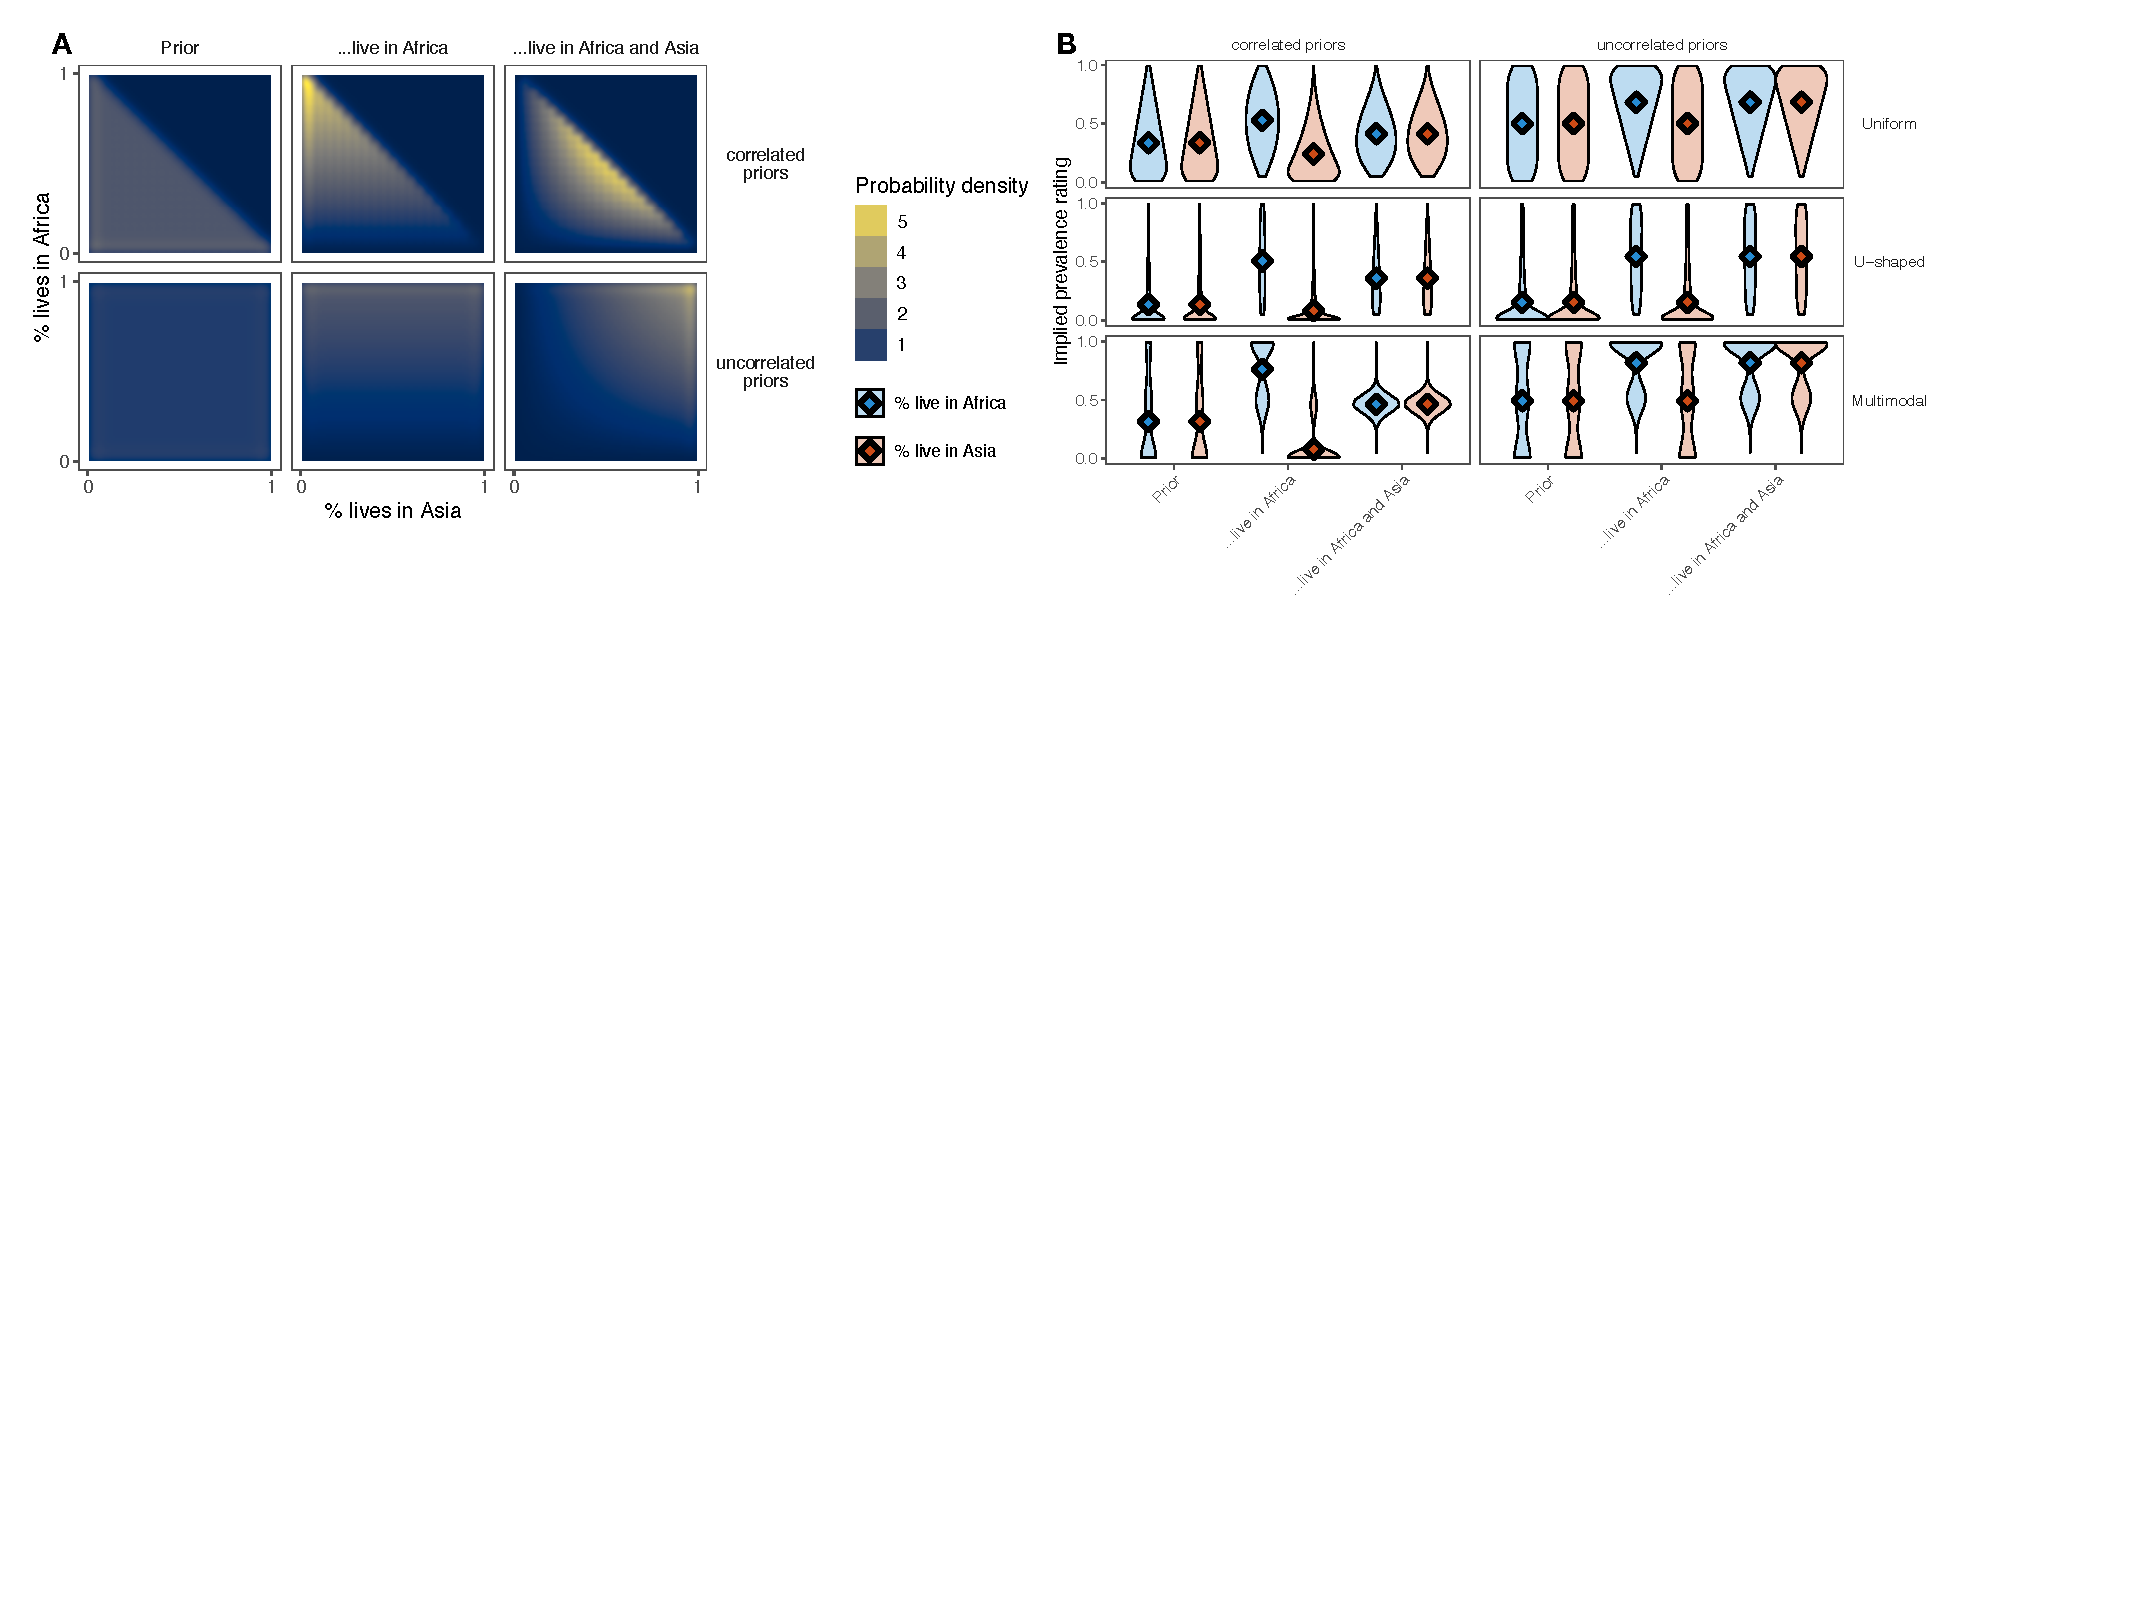
\includegraphics[width=1\textwidth]{model}
%    \vspace{-1cm}
  \caption{Model's sequential interpretation of ``Elephants live in Africa\ldots and Asia.'' A: Correlated priors reflected in the joint probability distribution over two features result in a mutual exclusivity inference. When the model hears only ``\ldots live in Africa'', it believes that probably all live in Africa (middle facet); when it hears they live in Asia as well, the model non-monotonically updates its beliefs about how many live in Africa. B: The mutual exclusivity inference holds for priors of different shapes and never holds if the prior knowledge about the two features is uncorrelated. Points show means of the distributions.}
  \label{fig:model}
\end{figure*}

We extend a model for interpreting generics to incorporate an incremental processing mechanism that allows a listener to understand partial utterances.
The original model of \citeA{Tessler2019:genLang} interprets a generic utterance predicating a property of a category (``Elephants eat 300 pounds of food in a day'') as meaning that the prevalence $x$ (or probability) of the property given the category---$P($eats 300 lb. of food in a day$\mid$ is an elephant$)$---is greater than an \emph{a priori} uncertain threshold $\theta$.
The literal meaning of the generic---an uncertain threshold function, with uniform uncertainty over the threshold $P(\theta$)---combines with a listener's prior knowledge about the prevalence of the feature $P(x)$ within a relevant set of alternative categories (e.g., other animals) to compute a posterior distribution over prevalence $x$:
%
\vspace{-0.2cm}
\begin{equation}
P(x \mid u) = \int_{\theta} P(x, \theta \mid u)  d\theta \propto P(x) \cdot P(\theta) \cdot \delta_{\denote{u}(x, \theta)} 
\label{eq:L0}
\vspace{-0.15cm}
\end{equation}
\noindent where $\delta_{\denote{u}(x, \theta)}$ is the Kronecker delta function assigning a value of 1 for utterances that are literally true (in the case of a generic: where $x > \theta$) and 0 for utterances that are false.



%Eq.~\ref{eq:L0} is a model of a Bayesian listener interpreting a generic utterance.
%
% To interpret a generic about a conjunctive predicate such as ``Elephants live in Africa and Asia'', we assume the sentence gets parsed into:\footnote{
% It is also possible to parse the sentence as:
%  $[G_\theta i. \textnormal{ elephants}(i) \to \textnormal{live\_in}(\textnormal{Africa} \land \textnormal{Asia})]$, though in the case of mutually exclusive predicates (e.g., ``lives in Africa'' and ``lives in Asia''), this parse would yield a false statement. It is not obvious that the two parses make different predictions for non-mutually exclusive predicates (e.g., ``lives in Africa and eat bugs''), and so we assume the more encompassing parse in Eq. \ref{eq:sem}
% }
% \begin{equation}
% \begin{split}
% [G_\theta i. \textnormal{ elephants}(i)& \to \textnormal{live\_in}(\textnormal{Africa})] \land \\
% [G_\theta i. \textnormal{ elephants}(i)& \to \textnormal{live\_in}(\textnormal{Asia})] 
%
To interpret a generic with a conjunctive predicate such as ``Elephants live in Africa and Asia'', we assume the semantic representation:
% \footnote{It is also possible to parse the sentence as:
%  $[G_\theta x. \textnormal{ elephants}(x) \to \textnormal{live\_in}(\textnormal{Africa} \land \textnormal{Asia})]$, though in the case of mutually exclusive predicates (e.g., ``lives in Africa'' and ``lives in Asia''), this parse would yield a false statement. It is not obvious that the two parses make different predictions for non-mutually exclusive predicates (e.g., ``lives in Africa and eat bugs''), and so we assume the more encompassing parse in Eq. \ref{eq:sem}
% }
%\begin{equation}
%\begin{split}
$
[G_\theta x. \textnormal{ elephant}(x) \to \textnormal{live\_in}(\textnormal{Africa})] \land
[G_\theta x. \textnormal{ elephant}(x) \to \textnormal{live\_in}(\textnormal{Asia})] 
$
%\end{split}
%\label{eq:sem}
%\end{equation}
(see \citeA{Nickel2008} for supporting arguments).
%Consider our running example of ``Elephants live in Africa and Asia''.
A listener starts with a joint prior over the prevalence of the two properties (we denote variables associated with \emph{living in Africa} with subscript $r$ and \emph{Asia} with $s$): $P(\textbf{x}) = P(x_{r}, x_{s})$, which incrementally updates with each successive generic. 
The model can then interpret multiple generics in succession, using the posterior distribution over prevalence $P(\textbf{x} \mid u)$ (Eq.~\ref{eq:L0}) as the prior for the next utterance. 
\begin{equation}
P(\textbf{x} \mid u_{r}, u_{s}) \propto  \int_{\theta_s} \int_{\theta_r}P(\textbf{x}, \boldsymbol{\theta} \mid u_{r})  \cdot \delta_{\denote{u_{s}}(x_{s}, \theta_{s})} d\theta_r d\theta_s%\\
%		& \propto & P(\vec{x}) \cdot P(\vec{\theta}) \cdot \delta_{\denote{u_{Af}}(x_{Af}, \theta{Af})} 
\label{eq:L0a}
\end{equation}
\noindent where $P(\textbf{x}, \boldsymbol{\theta} \mid u_{r})$  is the posterior that results from hearing ``Elephants live in Africa'' given by Eq.~\ref{eq:L0}.

The predictions for a sequential understanding of ``Elephants live in Africa and Asia'' are shown in Fig.~\ref{fig:model}.
The model believes that almost all elephants live in Africa, when hearing the first part of the utterance (simulations assuming a uniform prior shown in Fig.~\ref{fig:model}A). 
What happens next depends upon the correlational structure of the prevalence prior: If the listener has prior knowledge suggesting the properties (living in Africa, living in Asia) are mutually exclusive (Fig.~\ref{fig:model}A top), they interpret the next part of the utterance (``...and Asia'') as indicating that some (perhaps half) of elephants live in Africa and other ones live in Asia. 
Without this correlation in the prior, the model ends up believing that most or all elephants live both in Africa and in Asia  (Fig.~\ref{fig:model}A bottom).
%The joint probability distribution $P(\textbf{x})$ requires a correlational structure (i.e., knowledge of the mutual exclusivity of properties) in order to derive the inference that 50\% live in Africa and 50\% live in Asia; notably, the model first believes that almost all elephants live in Africa, when hearing the first part of the utterances (simulations assuming a uniform prior shown in Fig.~\ref{fig:model}A). 
These inferences are robust to a variety of different prevalence prior distributions, so long as the prior has the necessary correlational structure (Fig.~\ref{fig:model}B shows predictions assuming a uniform, U-shape Beta, and mixture-of-Beta distributions).

%We test this prediction in a generic interpretation study using mutually exclusive (ME) and non mutually exclusive (NME) properties (Expt. 1). 

\begin{figure}
  \definecolor{darkgreen}{RGB}{0,100,0}
    \definecolor{lightgreen}{RGB}{144,238,144}
\tikzset{sibling distance=-3pt, level distance=16pt}
  \centering
\scriptsize
\begin{tabular}{cc}
  \hspace{-0.25cm}
 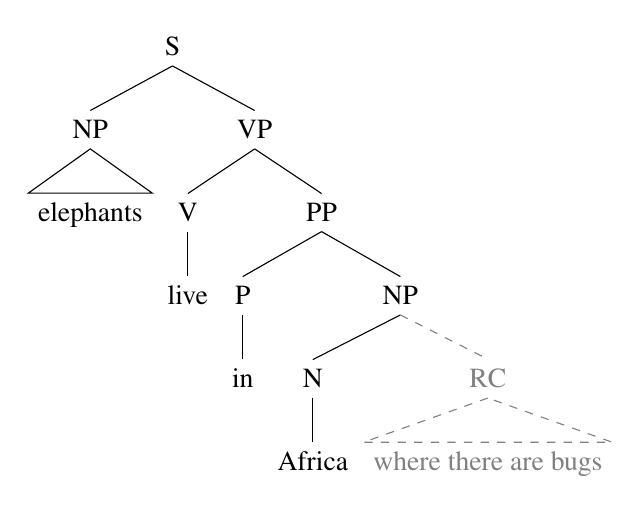
\begin{tikzpicture}
	        \Tree [.S [.NP \edge[roof]; elephants ]
	                  [.VP [.V live ] [.PP [.P in ] [.NP [.N Africa ] \edge[color=gray, style=dashed]; [.{\textcolor{gray}{RC}} \edge[color=gray, style=dashed, roof]; {\textcolor{gray}{where there are bugs}} ] ] ] ] ]
                              \end{tikzpicture}
&\hspace{-1.25cm}
 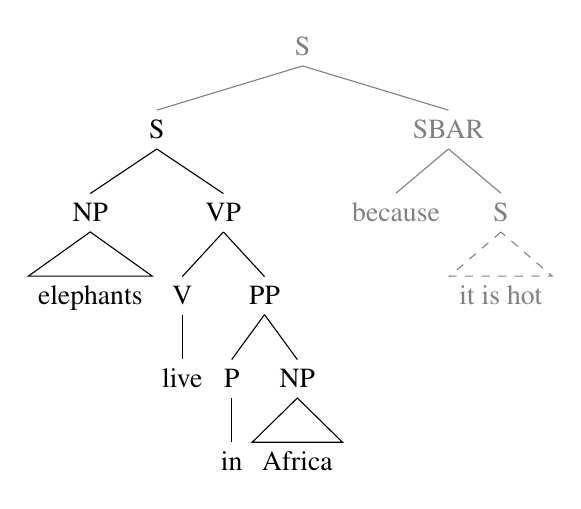
\begin{tikzpicture}[sibling distance=0pt]
	        \Tree [.{\textcolor{gray}{S}} \edge[color=gray]; [.S [.NP \edge[roof]; elephants ]
                [.VP [.V live ] [.PP [.P in ] [.NP \edge[roof]; Africa ] ] ] ]
                \edge[color=gray];
                [.{\textcolor{gray}{SBAR}} \edge[color=gray];  \textcolor{gray}{because} \edge[color=gray]; [.{\textcolor{gray}{S}} \edge[color=gray,style=dashed, roof]; {\textcolor{gray}{it is hot}} ] ] ]
                              \end{tikzpicture}
  \\
    \hspace{-0.5cm}
      \begin{tikzpicture}[sibling distance=0pt]
	        \Tree [.S [.NP \edge[roof]; elephants ]
	                  [.VP [.V live ] [.PP [.P in ]
	                       	[.NP [.NP Africa ] 
                                 \edge[color=darkgreen]; [.\textcolor{darkgreen}{Conj} \textcolor{darkgreen}{and} ]
		                       	\edge[color=lightgreen, style=dashed]; [.\textcolor{lightgreen}{NP}  \edge[color=lightgreen, style=dashed, roof]; \textcolor{lightgreen}{Asia} ]] ] ]]
	\end{tikzpicture}
    & \hspace{-1cm}
\begin{tikzpicture}[sibling distance=0pt]
	        \Tree [.S [.NP \edge[roof]; elephants ]
	                  [.VP [.VP \edge[roof]; {live in Africa} ]
                               \edge[color=darkgreen]; [.\textcolor{darkgreen}{Conj} \edge[color=darkgreen]; \textcolor{darkgreen}{and} ] 
				\edge[color=lightgreen, style=dashed]; [.\textcolor{lightgreen}{VP}  \edge[color=lightgreen, style=dashed, roof]; \textcolor{lightgreen}{eat bugs}
				] ] ]
                              \end{tikzpicture}
  \end{tabular}
   
\caption{Incremental parse trees and syntactic expectations for upcoming conjunct properties in generic predication.  The string prefix ``Elephants live in Africa\ldots'' is compatible with a variety of continuations, including the four listed above.  The next word, ``\textcolor{darkgreen}{and}'', rules out continuations like those the top row (depicted in gray) and sharpens expectations around a conjunct at potentially different structural levels (light green).  Probabilistic renormalization implies that an upcoming conjunct mutually exclusive with the first conjunct becomes more likely when ``and'' is encountered, driving the strong incremental predictions depicted in Fig.~\ref{fig:incremental}.}
\label{fig:trees}
\end{figure}


When processing a conjunctive phrase, listeners may form expectations about the complete utterance even before the sentence is over. 
For example, when a speaker reaches the word \emph{and} in ``Elephants live in Africa \emph{and}'', she has two syntactically distinct options available to her when completing the sentence: She could continue with a noun phrase (e.g., ``and Asia'') or a verb phrase (e.g., ``and eat bugs''; Fig.~\ref{fig:trees}).
Each of these continuations would imply different inferences about the prevalence of elephants in Africa.\footnote{
	Of course, it is possible to continue with a verb phrase about a mutually exclusive property such as ``\ldots live in Africa and live in Asia'' as well as continue with a noun phrase about a non-mutually exclusive property (e.g., ``\ldots eat figs and nuts''). Our focus is on the fact that a speaker can continue the conjunction with a mutually exclusive or non-mutually exclusive property, which in the cases we consider, are highly correlated with NP~vs.~VP coordination.
}
If listeners parse and interpret utterances incrementally at the level of individual words, then we would expect their inferences about the prevalence of elephants in Africa to represent a mixture of the inferences derived from these two possible continuations, which can be represented by conditional probabilities of the full utterance given the sentence fragment heard $f$:

\vspace{-0.3cm}
\begin{equation}
P(x \mid f) = \sum_{u'} P(x \mid u') P(u' \mid f) 
\label{eq:L0a}
\vspace{-0.3cm}
\end{equation}

If, however, listeners do not derive incremental interpretations at each moment, but instead wait for meaningful pieces of an utterance (e.g., content words like \emph{Asia}) to compute interpretations, then we would not expect such an intermediate degree of interpretation: ``Elephants live in Africa and\ldots'' should mean the same thing as ``Elephants live in Africa\ldots'' (Fig.~\ref{fig:incremental}). 
We test this prediction in Expt.~2 using a gating paradigm in the spirit of \citeA{Grosjean1980}.
%We consider the case of listeners encountering the coordinating connection ``and'' in the predicate of a generic sentence. 
%For simplicity, we assume that speakers can continue a sentence such as ``Elephants live in Africa and'' with either an NP coordination with a mutually exclusive property (``Asia'') or VP coordination with a non-mutually exclusive property (``eat 300 pounds of food a day'').\footnote{
%	Of course, NP-coordination with non-mutually exclusive properties is possible (e.g., ``eat figs and nuts''). 
%	Our focus in this paper is on the fact that a speaker can continue the conjunction with a mutually exclusive or non-mutually exclusive property, which in the cases we consider, are perfectly correlation with NP~vs.~VP coordination.
%}


%In order to model incremental interpretations of the utterance, we extend this model to allow a listener to form expectations about plausible continuations from sentence fragments $f$.
%To do this, we assume that a listener has probabilistic expectations about how a speaker will choose to complete the utterance given a fragment $P(u' \mid f)$.










\begin{figure}[t]
  \centering
    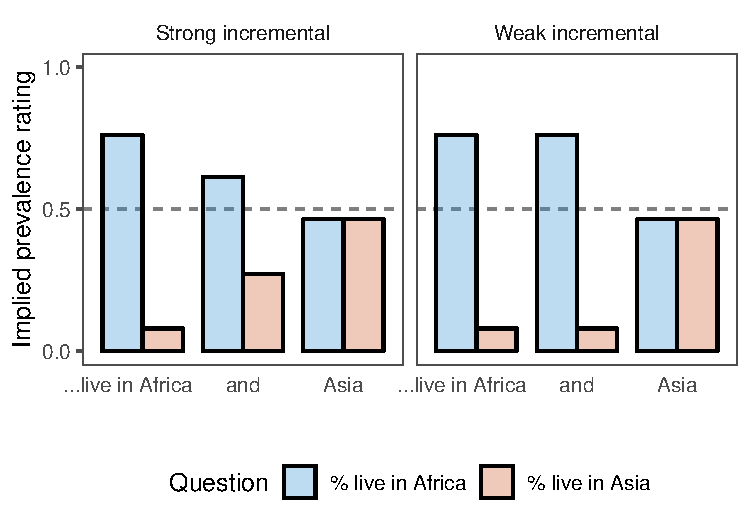
\includegraphics[width=0.5\textwidth]{incremental}
%    \vspace{-1cm}
  \caption{A model that incorporates syntactic expectations at the level of individual words (\emph{strong incremental}) predicts intermediate mutual-exclusivity inferences part-way through the conjunction (at ``and''), whereas a model that waits for content-words (\emph{weak incremental}) to begin to understand the utterances does not show a difference in expected prevalence at the word ``and.''
%  Model interpretation of a conjunctive generic (``Elephants live in Africa and Asia''). A: Intuitive priors for marginal distributions of prevalence for living in Africa and living in Africa. B: Partial interpretation upon hearing utterance (“Elephants live in Africa . . .”). C: Full interpretation upon hearing the end of the sentence (``...and Asia''). Uncertainty about the threshold for generic sentences allows the listener to non-monotonoically update its beliefs about the prevalence of the feature in categories.
  }
  \label{fig:incremental}
\end{figure}


%Extending an analysis of generics to handle complex-predicates poses unique challenges.
%A sentence of the form ``Ks F and G'' introduces an ambiguity:
%
%\begin{enumerate}
%\tightlist
%\item $\denote{gen}(K) [F \land G]$
%\item $\denote{gen}(K) [F] \land \denote{gen}(K) [G]$
%\end{enumerate}


\section{Experiments}

We design two experiments to test the mutual exclusivity (ME) and incremental predictions of the model. 
Expt.~1 tests the ME predictions that ``Elephants live in Africa and Asia'' means roughly that half live in Africa and half live in Asia; this experiment also serves to validate the gating procedure we will employ in the second experiment. 
Expt.~2 is a pre-registered study that uses the gating paradigm to test the fine-grained incremental predictions of the model.
The experiments and full-list of materials can be viewed at \url{https://tinyurl.com/elephants-cogsci}.

%; we compare interpretations for these conjunctive generics with those of conjunctive generics about non-mutually exclusive (NME) properties (e.g., ``Elephants live in Africa and eat 300 lb. of food in a day''). 
%Experiment 2 is a conceptual replication using an adaptation of a gating paradigm \cite{Grosjean1980} which also controls for asking about two properties previously mentioned using a conjunctive generic sentence. 
%Sample size, participant exclusion criteria, and primary planned analyses for all experiments were pre-registered on OSF \red{(url removed for blinding)}.


\begin{figure*}[h]
  \centering
    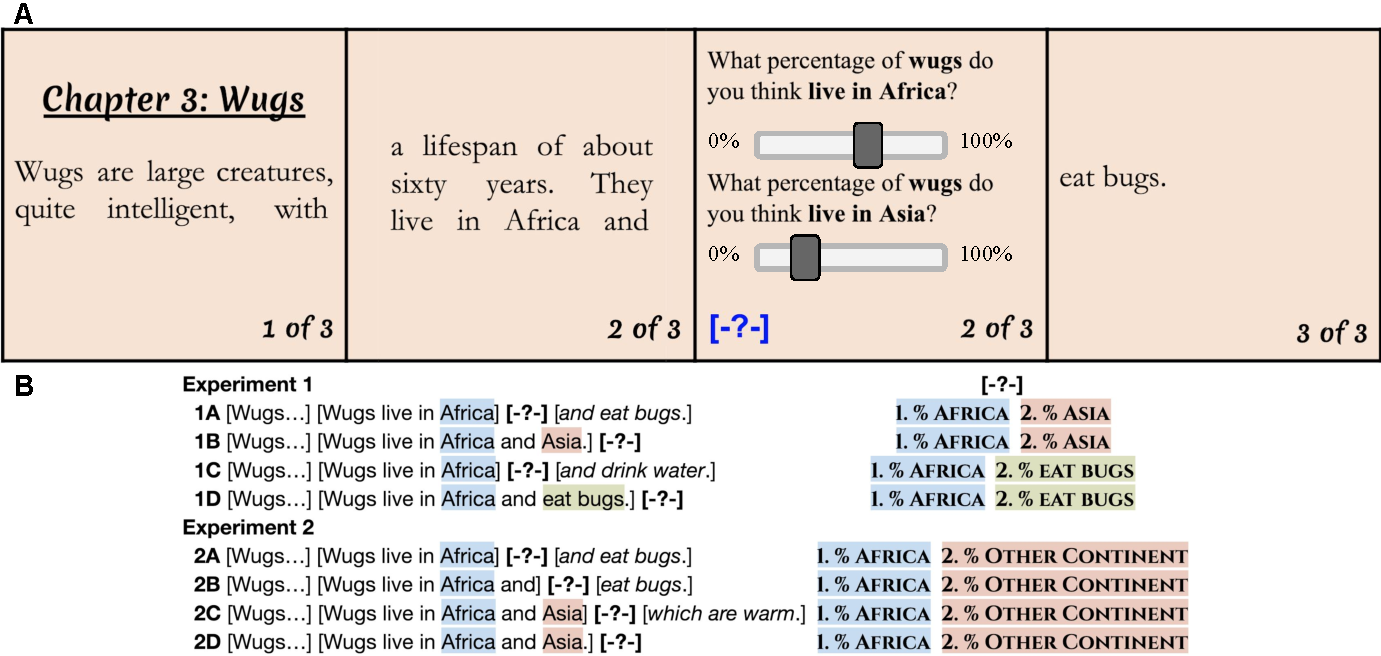
\includegraphics[width=1\textwidth]{design}
%    \vspace{-1cm}
  \caption{Overview of experiments. Experiment 1 compared interpretations of generics about mutually exclusive (ME) properties and non-mutually exclusive properties (NME), by asking about the implied prevalence of the two ME properties. Experiment 2 queried for partial interpretations of conjunctive generics by interrupting with a question ([-?-]) after the first property;  in addition, Expt. 2 measure implied prevalence for the two NME properties (e.g., \% eat bugs). Experiment 3 queried for partial interpretations by interrupting at three different points in the sentence. }
  \label{fig:design}
\end{figure*}

\subsection{Experiment 1: Mutual exclusivity inference}

%\subsubsection{Methods}
\subsubsection{Participants}
We recruited 27 participants through Amazon's Mechanical Turk.
Participants were restricted to those with verified U.S. IP addresses and had at least a 95\% work approval rating. 
The study took about 10 minutes and participants were compensated \$1.50.

\subsubsection{Materials}

Participants read a storybook, consisting of several chapters about aliens and animals on a far-away planet.
% without any larger narrative (each chapter concerned different categories or characters).
Each chapter contained a short paragraph of text presented across 2--4 screens, with participants having to click a button to ``turn the page'' (Fig.~\ref{fig:design}A).
A chapter introduced one or a few novel categories (e.g., \emph{wugs}) and semi-novel properties (e.g., \emph{live on the continent of Caro}).
Critical trial chapters ended with a generic sentence about conjunctive properties, which differed only in whether the second property was mutually exclusive with the first (\emph{conjunct type}): ``Glippets live on the continent of Caro and \emph{on the continent of Este} (ME) /  \emph{enjoy the sunshine there} (not mutually exclusive; NME).''

The other content of the chapter supported the mutually exclusive interpretation of the properties, when the properties were not \emph{ipso facto} mutually exclusive. For example: 

\vspace{-0.1cm}
\begin{quote}
\small
Krens are a tribe of the aliens that live on the continent of Benli. Animals like stups, four-legged creatures with large antlers, are a resource for the Krens. Stups roam all over the windy highlands of Benli, far from the oceans. Krens are stup-herders and \emph{fishermen} / \emph{incorporate stups into their religion}.
\end{quote}
\vspace{-0.1cm}


Conjunct type (ME~vs.~NME) was manipulated within-participants and within-items. 
In addition to the critical items, there were 14 filler chapters, which concerned similar content to the critical chapter but which explicit quantifiers (\emph{most}, \emph{all}, or \emph{none}) to predicate properties of categories. 






%We used \red{10} critical chapters (items), each which could be assigned to one of two experimental conditions.
%A given chapter in the two experimental conditions differed only in the information present on the final screen of a chapter.
%The penultimate screen of all critical trials ended with the beginning of a conjunctive sentence that was broken up immediately before the ``and'' in the sentence \red{(Figure); e.g., ``They ascribe to the Caboo religion'')}. 
%Text on the page was fully-justified so that the final word on a page always appeared in the bottom-right corner of the screen, giving the appearance that the page naturally ended at that word.
%In the \emph{relevant conjunction} condition, the continuation of the sentence (final screen) was a property that was anti-correlated (or, somewhat mutually exclusive) with the property on the preceding page (e.g., ``and the Daith religion''). 
%In the \emph{irrelevant conjunction} condition, the continuation was a property that was unrelated to the property on the preceding page (e.g., ``...and follow a strict code of laws.''). 
%In addition, we had 5 filler trials which appeared similar to the \emph{irrelevant conjunction} cases.

%\begin{table*}[t]
%\small\addtolength{\tabcolsep}{-5pt}\renewcommand{\arraystretch}{1.1}
%\begin{tabular*}{\textwidth}{p{5.5cm}p{6.5cm}p{6cm}}
%\hline
%Property & Mutually Exclusive (ME) & Non-Mutually Exclusive (NME) \TBstrut\\ \hline
%ascribe to Cabooism & ascribe to Daithism & pray three times a day \Tstrut\\ 
%live on the continent of Caro & live on the continent of Este & graze on the tall grasses \\ 
%have territories at tops of tall mountains & have territories at bottom of deep canyons & watch over low-lying regions during the day \\ 
%plant fujusi & plant soroneeks & spray fields with naturally-occurring fertilizer \\ 
%build nests in gluers & build nests in droops & store tree-bark in them for safe keeping \\ 
%are stup-herders & are fishermen & sing songs to the stups to help them relax \\ 
%have long wings & have short wings & have sharp claws \\ 
%wear wutsats around their heads & wear krevnors around their heads & carry sticks with them \\ 
%chew on xorfun bark & chew on tunkel bark & jump up and down in circles \\ 
%carry their young in guklags & carry their young in trullets & are very protective \\ 
%are part of the Tinnoclan & are part of the Farzaguild & sell their baskets in the Warfi marketplace \\ 
%hibernate in fallen logs & hibernate in abandoned burrows of other animals & give birth twice a year \\ 
%has bumpy skin & has smooth skin & has a sour taste \Bstrut\\
%\hline
%\end{tabular*}
%\caption{Stimuli used in Experiments 1 \& 2. }
%\end{table*}


\subsubsection{Procedure}
Participants were told they would be reading a storybook and be asked questions at some point in each chapter. 
Questions were all of the same type, an \emph{implied prevalence} question \cite{Gelman2002, Cimpian2010} that read: ``What percentage of Ks do you think F?'', where K represents a category and F a feature. 
Responses were recorded using a 101-pt slider bar with end-points labeled 0\% and 100\%, with the exact value selected appearing above the slider. 
Participants were familiarized with the response variable in a practice trial, where they were asked to report how many \emph{dogs bark}, \emph{birds are male}, \emph{cats get cancer}, and \emph{lions lay eggs}. 
We used these questions to encourage participants to use the full range of the response scale as well as to serve as a comprehension check. 

Following these instructions and practice questions, participants read the storybook.
% consisting of \red{16} paragraphs we refer to as \emph{chapters} (items), each of which spanned 2 - 4 screens of text which spanned 2 - 4 lines on the screen. 
Within each critical chapter, two questions appeared either at the end of the chapter or interrupting the chapter right before the final page.
The interrupting question came in the middle of a conjunctive generic, but before the word ``and'', so it was not immediately clear that the sentence would continue with a conjunction.
The questions asked about the mentioned property (e.g., Africa) and either a mutually exclusive property (Asia) or a nonmutually exclusive property (e.g., ``eats bugs''); the chapter then concluded with a conjunction about an unmentioned, nonmutually exclusive property (Figure \ref{fig:design}B).
The order that the questions appeared on the screen was randomized on each trial.
If the question came at the end of the chapter, the critical conjunctive generic either finished with a mutually exclusive or nonmutually exclusive property; whatever property was used as the conjunct was also used as the second question on the question screen ([-?-]).
For filler trials, the two questions were asked about two properties that were conveyed using the same quantifiers (i.e., properties both described with \emph{all}, \emph{most}, or \emph{none}).

The story book consisted of a total of 21 chapters, which included 8 examples of the mutually exclusive conjunctions (4 interrupted, 4 uninterrupted) and 4 examples of the nonmutually exclusive conjunctions (2 interrupted; 2 uninterrupted); in addition, there were 8 filler trials involving quantifiers (4 interrupted, 4 uninterrupted). 
The experiment began with 2 filler trials, and the other trials were presented in a random order with the constraint that no two critical trials were presented back-to-back. 
At the end of the storybook, participants completed a memory check question where they had to select all the facts they had learned in the story from a list of 10 (5 real, 5 distractor); in addition, participants were asked to explain, in very broad terms, what the experiment was about.

%right before the conjunction ``and'' (Figure \ref{fig:design}A, but with ``and'' appearing on page 3 rather than page 2). 
%This was to provide a comparison to another property that was also mentioned in a conjunctive generic sentence but for which ME inferences were not expected.



%The text of a chapter mostly composed of generic sentences about novel categories (e.g., ``Glippets are intelligent creatures''), though some sentences mentioned specific fictional characters (``Wint lived a long time ago in the mountains.'').

%Eaach chapter of the storybook was on



\subsubsection{Results}

%\begin{figure}[h]
%  \centering
%    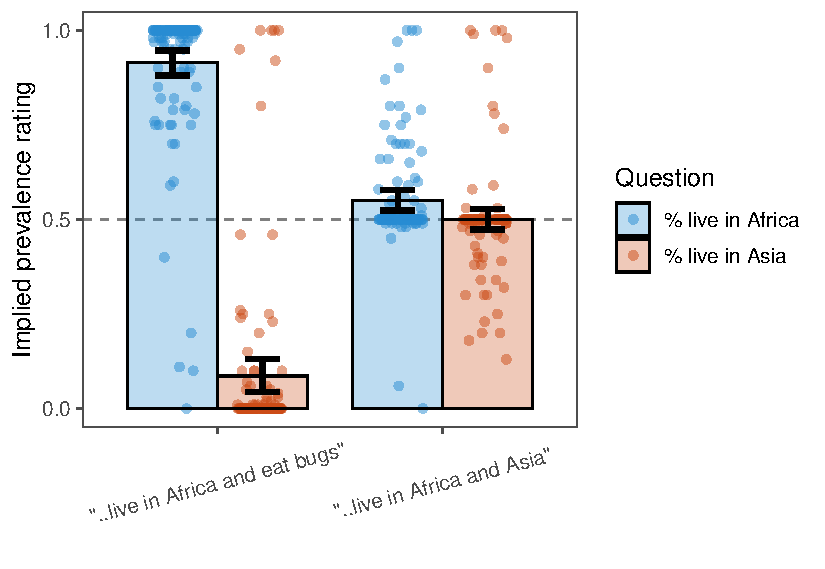
\includegraphics[width=0.5\textwidth]{expt1_summary}
%%    \vspace{-1cm}
%  \caption{Experiment 1 results. Participants' ratings of the percentage of a category with a property (color) upon hearing a conjunctive generic either with non-mutually exclusive properties (left) or mutually exclusive properties (right). Error-bars denote bootstrapped 95\% confidence intervals; points are individual responses. \mh{does mutual exclusivity fail for some people?}}
%  \label{fig:expt1}
%\end{figure}




11 participants were excluded for either failing to respond accurately to all of the practice trials or  failing to respond accurately to at least 7 of the 10 memory check prompts (same exclusion criteria for all experiments).
We describe the results from the perspective of the running example of ``Elephants live in Africa and Asia'', but the experimental stimuli used novel categories and relatively novel properties.
%, or responded randomly to the explanation question in a way that suggested they were a bot (e.,g., ``nice experiment'' in all caps; often if they failed the explanation trial, they failed at least one of the two other checks).
 
Reading only that ``Elephants live in Africa\_\_'' led listeners to believe that all elephants lived in Africa and that none lived in Asia , whereas if the sentence finished ``\_\_and Asia'', listeners inferred that roughly half live in Africa and half live in Asia (Figure \ref{fig:expt2}A). 
The same pattern is not observed for properties that are not construed as mutually exclusive, where hearing about the second property only increases participants' degree of belief in the property applying (Figure \ref{fig:expt2}B).
In addition, when answering a question about the unmentioned property, participants rated the prevalence of the mutually exclusive property as close to 0\% whereas a non-mutually exclusive property was rated as somewhat prevalent (third green bar).
The results replicate intuitions about how ``Elephants live in Africa'' should be interpreted using an interrupting question.
Our comparison to the non-mutually exclusive condition shows that the results cannot be attributed to the very act of being asked about two properties mentioned in a conjunctive generic sentence.
%\mh{should i run a regression model here or is it unncessary?}


% (posterior mean estimate and 95\% credible interval: $\beta = -2.11 [-1.2, -3.3]$; Figure \ref{fig:expt1}).  



%Our primary analysis is whether implied prevalence estimates to the first property in a conjunctive generic sentence (e.g., the \% of elephants that live in Africa) changes as a function of the second property.
%In particular, we predict that implied prevalence estimates for the first conjunct will be higher when the second conjunct is not mutually exclusive than when it is ME. 
%To test this prediction, we constructed a Bayesian mixed-effects regression model predicting implied prevalence ratings to the first conjunct (e.g., \% live in Africa) as a function of the second conjunct that appeared in the sentence.
%%\footnote{
%% We model the raw data as being generated from a 0- and 1-inflated beta distribution. This allows us to keep the data in a raw format (as %slider bar ratings between 0-1, including the endpoints).
%%}
%In addition, we included by-item and by-participant random-effects of intercept and effect of condition manipulation.
%Consistent with our prediction, participants responded that substantially fewer elephants lived in Africa when they read ``Elephants live in Africa and Asia'' then when they read ``Elephants live in Africa and eat 300 lb. of food a day'' (posterior mean estimate and 95\% credible interval: $\beta = -2.11 [-1.2, -3.3]$; Figure \ref{fig:expt1}).  
%
%\subsection{Experiment 2: Interrupting questions}
%
%In Expt.~1, we observed that the nature of the second conjunct in a conjunctive generic sentence can influence inferences about the prevalence of the first conjunct.
%Here, we test for a potential confound in the design of Expt.~1: Whenever participants provided prevalence estimates for two properties that they had read about in a conjunctive generic, the inference was that they were mutually exclusive. 
%Here we provide a control wherein participants can provide ratings about two properties previously mentioned in a conjunctive generic but which are not  mutually exclusive. 
%In addition, we aim to replicate the pattern of Expt.~1 using a gating technique wherein participants are queried part-way through a sentence. 
%
%\subsubsection{Participants}
%
%We recruited \red{N} participants through Amazon's Mechanical Turk.
%This number was arrived at with the aim of collecting \red{N} participants' data who passed the attention checks.  
%Participants were restricted to those with verified U.S. IP addresses and had at least a 95\% work approval rating. 
%
%\subsubsection{Materials and procedure}
%
%The materials were the same as used in Expt.~1 and the procedure was identical except for the critical trials.
%Each critical trial either had a question at the end of the chapter (as in Expt.~1; \emph{uninterrupted condition}) or immediately before the final page of the chapter (\emph{interrupted condition}).
%For the interrupted conditions, the critical sentence broke at the page-break before the conjunction (e.g., ``Elephants live in Africa\_\_'', where \_\_ denotes the page break). 
%For the uninterrupted conditions, the question appeared at the end of the chapter.
%Each chapter ended with a generic sentence about conjunctive properties, which differed only in whether the second property was mutually exclusive (ME) with the first (\emph{conjunct type}): ``Glippets live on the southern continent of Caro and \emph{on the northern continent of Este (ME) /  enjoy the sunshine there (nME).}''

%E2: AF&AS / AF/  AF&NME[Qnme] / AF[Qnme]


%\subsubsection{Results}

\begin{figure}[h]
  \centering
    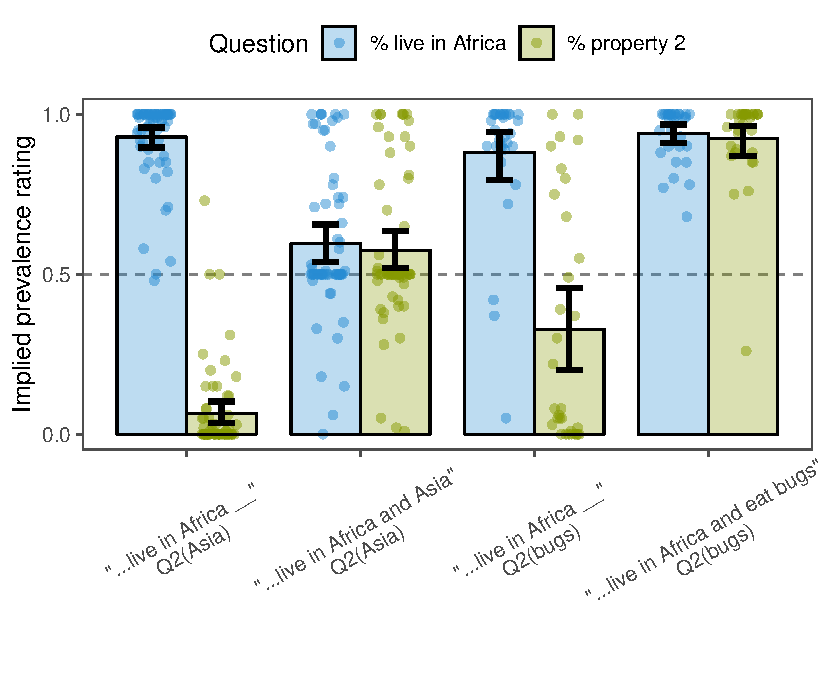
\includegraphics[width=0.5\textwidth]{expt2_summary}
%    \vspace{-1cm}
  \caption{Experiment 1 results.  Participants rate prevalence for mentioned property (\% live in Africa) and ``Property 2'', either the mutually exclusive property (left two bars) or non-mutually exclusive property (right two bars). ``\_\_'' indicates the question appears mid-sentence. Error-bars denote bootstrapped 95\% confidence intervals.}
  \label{fig:expt2}
  \end{figure}


\subsection{Experiment 2: Strong incrementality}

In Expt.~1, we demonstrated that the mutually-exclusive inference effects can be measured using a gating paradigm wherein participants are queried for their beliefs part-way through a sentence. 
Here, we exploit this paradigm to test the strong incremental processing predictions of the model, wherein syntactic expectations can modulate the interpretations of generic sentences in a fine-grained manner. 

\subsubsection{Participants}

We recruited 108 participants through Amazon's Mechanical Turk.
This number was sufficient to collect 80 participants' data who passed the attention checks.  
Participants were restricted to those with verified U.S. IP addresses and had at least a 95\% work approval rating. 
Sample size, participant exclusion criteria, and primary planned analyses for this experiment was pre-registered on OSF \red{(url removed for blinding)}.

\subsubsection{Materials and procedure}

%The majority of the critical trial materials were the same as those used in Expt.~1.
The critical conjunctive generics used in Expt.~1 involved conjunctions of different grammatical categories, though always with the same syntactic types (e.g., ``ascribed to the Caboo religion and the Daith religion'' is a conjunction of two determiner phrases). 
We modified the critical conjunctive generics to involve mostly conjunction of two noun phrases (e.g., ``ascribe to Cabooism and Daithism'') in order to strength correlation between the NP-conjunction and mutual exclusivity. 
The fillers were modified to introduce page breaks immediately before and immediately after conjunctions (the word ``and'') in order to raise participants' expectations that a sentence might be broken at a conjunction.
We used additional examples of the Uninterrupted ME condition of Expt.~1 (``live in Africa and Asia.'') to raise participants' expectations about of ME continuations.
Half of these filler trials had page breaks immediately before the ``and'' and half immediately after.

On critical trials, questions always interrupted the chapter, appearing right before the last page.
On the question screen, the page number of the penultimate page remained on the screen to provide an additional cue to participants that the chapter was not complete (Figure \ref{fig:design}A).
There were three kinds of critical trials corresponding to the point at which the page break occurred in the conjunctive generic sentence: after ``Africa'', after ``and'', or after ``Asia'' (Figure \ref{fig:design}). 
When participants did not see the full conjunctive property before the question (conditions INT A and A\&), the sentence continued after the question with a non-mutually exclusive property (e.g., ``Africa and eat bugs''), so as to not give the impression that the participant was being tricked. 

Finally, we changed the question about the second property (\% live in Asia) to ask about ``some other X'', where X was the kind of property that was mentioned in the first conjunct (e.g., ``live on some other continent'').
This change was introduced to raise the plausibility that a second, mutually exclusive property was possible while not explicitly naming a particular property, which would be pragmatically odd given that the property is unmentioned in the INT A and INT A\& conditions. 
In making this change, we dropped 3 stimuli because they did not lend themselves naturally to this question frame.
 \subsubsection{Results}
 
\begin{figure}[h]
  \centering
    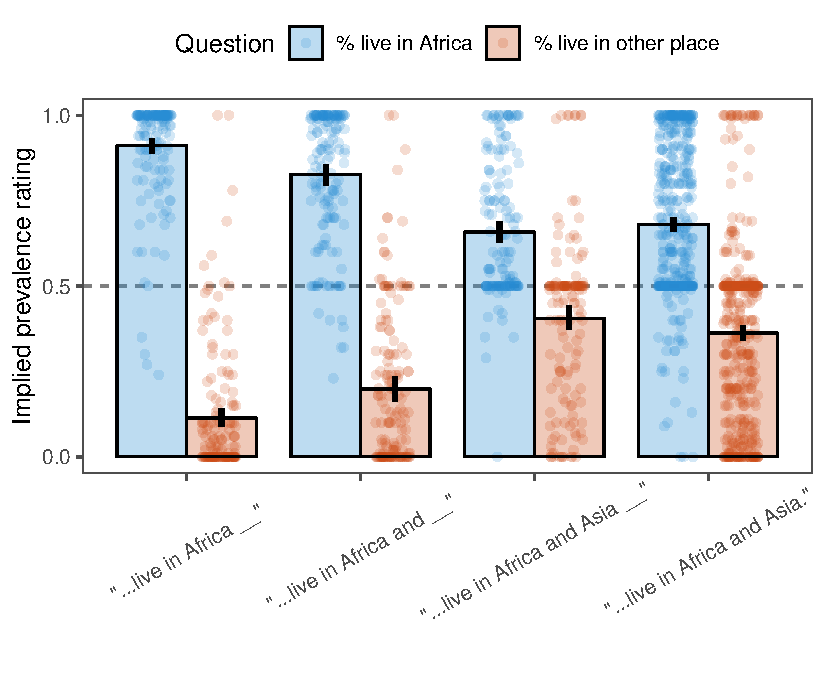
\includegraphics[width=0.5\textwidth]{expt3_summary}
%    \vspace{-1cm}
  \caption{Experiment 2 results. Participants are interrupted at various stages of the sentence (either after \emph{Africa}, \emph{and}, or \emph{Asia}) to be asked about the prevalence of \emph{living in Africa} and \emph{living in some other place}, or asked at the end of the sentence (right-most bars). When participants are interrupted before the second conjunct (\emph{Asia}), the sentence continues with a non-mutually exclusive property. Error-bars denote bootstrapped 95\% confidence intervals.}
    \label{fig:expt3}
  \end{figure}
  
% \mh{Expt 3: 
% - ``live in Africa.'' condition?
% - ``live in Africa.'
% }
% 

28 participants were excluded for either failing at least one of the two attention checks.
To test our main prediction, we constructed a Bayesian mixed-effects regression model predicting implied prevalence ratings to the first conjunct (e.g., \% live in Africa) as a function of the point in the sentence in which participants were queried. 
In addition, we included by-item and by-participant random intercepts and slopes. 
The regression model was created in Stan (http://mc-stan.org/) accessed with the brms package \cite{burkner_brms_2017}.


Replicating the findings of Expt.~1, when participants only read that ``Elephants live in Africa'', they tended to infer that almost all lived in Africa. 
When they read that ``Elephants live in Africa and Asia'', they tended to infer that the distribution was close to 50\%-50\%.\footnote{
Note that participants, on average, infer the prevalence is higher in this condition than 50\% for \emph{Africa}. 
This is likely the result of asking about ``some other place'', which is substantially less specified that asking about a particular mentioned property.  Still, many participants responded exactly 50/50.
}
Finally, as predicted by a strong version of incremental processing, participants began to anticipate a mutually-exclusive conjunct when only the word ``and'' was mentioned, as evidenced by their implied prevalence ratings being substantially less for the ``..live in Africa and\_\_'' condition than the ``live in Africa'' condition (posterior mean estimate and 95\% credible interval: $\beta = -0.08 (-0.13, -0.04)$).
In addition, these ratings were substantially higher than when the full conjunctive predicate was present ``..live in Africa and Asia'' ($\beta = 0.17 (0.12, 0.23)$  (Figure \ref{fig:expt3}).
Thus, we find that the participants' implied prevalence ratings of how many elephants lived in Africa monotonically decreased as a function of how many words of the conjunctive predicate they were allowed to see. 
These results suggest that listeners begin to draw pragmatic interpretations of generics before the end of the sentence and even in the absence of additional content words. 

%%\footnote{
%% We model the raw data as being generated from a 0- and 1-inflated beta distribution. This allows us to keep the data in a raw format (as %slider bar ratings between 0-1, including the endpoints).
%%}

\section{Discussion}

Generic sentences exhibit extreme sensitivity to context that make it difficult to precisely define what a single generic conveys. 
``Elephants live in Africa and Asia'' means neither that \emph{most elephants live in (both) Africa and Asia} nor that \emph{Most elephants live in Africa, and most elephants live in Asia}.
Here, we empirically measured interpretations of generics about conjunctive predicates, building on the observation of \citeA{Nickel2008} of the range of troubling examples for quantificational views of generics.
Notably, the uncertain threshold model of \citeA{Tessler2019:genLang} accounts for such conjunctive generics seamlessly: An underspecified threshold can be updated as more information comes in, and is sensitive to prior beliefs regarding compatibility of the conjunct properties.

We extended that model to include syntactic expectations, and found evidence for the strongest form of incremental syntactic processing, wherein beliefs are continually updated based on expectations of how a sentence will continue. 
The fact that generic language understanding can be modulated simultaneously by correlations in background knowledge and syntactic expectations calls for a tighter coupling between models of syntactic processing \cite{Levy2008}, pragmatic language understanding \cite{Goodman2016}, and intuitive theories \cite{tenenbaum2011grow}. 

It remains an open question, however, how specific the effects observed in this paper are to generics as opposed to quantification more generally. 
For example, it appears that, in some contexts, one can use \emph{most} to convey similar mutually exclusive conjunctions: ``Elephants are the largest land animal on Earth and are one of the gentlest creatures. Most live in Africa and Asia but are brought to other places for the entertainment of humans.''\footnote{
Example from https://www.theodysseyonline.com/want-to-ride-an-elephant
}
Further work is needed to determine the felicity and interpretation of such utterances.


%The uncertain threshold model of \citeA{Tessler2019:genLang} models the interpretation of conjunctive generics about mutually exclusive properties such as ``Elephants live in Africa and Asia'' as incrementally updating the threshold beyond which the property holds (generically) in the category (see Model Predictions). 
%The model interprets the sentence as the conjunction of two full-blown generic sentences (``Elephants live in Africa, and elephants live in Asia''). 
%This phenomenon, however, appears as the inverse of the Free Choice effect, wherein listeners apply a conjunctive interpretation (``and'') to a disjunction (``or''), as in ``You can have ice cream or cake''. 
%Thus, an alternative account to the incremental, threshold updating model proposed here is that conjunctive generics about ME properties are the result of a similar kind of pragmatic inference one would use for the Free Choice account. 

%One way to potentially disambiguate the reverse-Free Choice from the incremental threshold updating model would be to investigate quantifier sentences which have a fixed-meaning (e.g., ``Most'' means roughly more than half).


% discussion
% interactivity between levels of context: here, knowledge of syntax and knowledge about properties
% how specific to generics are these findings vs. quantification generally? or there judgment differences?


%The availability of a computational model of generic language understanding permits natural extensions to incorporate other aspects of language understanding. 
%Coupling a modified gating paradigm \cite{Grosjean1980} with an implied prevalence task from the psychology of generics literature \cite{Gelman2002, Cimpian2010} allowed us to probe incremental understanding of generics. 
%We found evidence for a strong form of incremental processing, wherein beliefs are updating continuously even in the absence of content words.

%It is largely agreed that the context-sensitivity of generics needs to be accounted for at the level of individual properties in a particular context \cite{Nickel2008, Nickel2016, Sterken2015} as opposed to a purely more general framework where generics about different kinds of properties get ascribed different meanings \cite<e.g.,>{Prasada2013, Leslie2008}.
%Here we show that in fact the same property (``lives in Africa'') can be understood in two different ways when presented in a generic sentence. 
%When listeners hear that ``Elephants live in Africa'', they tend to think all elephants live in Africa; when they hear that ``Elephants live in Africa and Asia'', the implied prevalence of those living in Africa is quite lower. 
%This phenomenon bears some similarity to the \citeA{Nickel2008}'s ``Dobermans have pointy ears'', which in a context of dog-breeders is entirely acceptable, but not so in a discussion of dog genetics (Dobermans are born with floppy ears and breeders clip their ears to make them pointy).
%The unifying thread is that the same generic sentence can have dramatically different interpretations depending on the context. 
%Thus, the work here moves us one step closer to developing a unified treatment of the ways in which context can affect the meaning of generics.



%In Expt.~3, we manipulated syntactic expectations by providing both additional information about the two mutually exclusive properties as well as additional fillers which contained conjunctive generics about ME properties. 
%We find suggestive evidence that syntactic expectations can guide incremental pragmatic understanding of generic sentences. 
%Methodologically, it is possible that either one of our context manipulations (e.g., highlighting two salient properties to participants) would be sufficient to impact listeners' syntactic expectations for continuations of conjunctive predicates.
%It is also an open question what are listeners' baseline levels of syntactic expectations about conjunctions in these environments. 
%We are also actively investigating participants' baseline level of syntactic expectations using a cloze test.






%\section{Acknowledgments}
%
%We thank Karen Gu for her assistance in stimuli creation and experiment implementation.


\bibliographystyle{apacite}

\setlength{\bibleftmargin}{.125in}
\setlength{\bibindent}{-\bibleftmargin}

\bibliography{elephants}


\end{document}
